\subsection{Reactivity}
Asymptotic resilience governs the long-term rate of recovery. However, in the short term, perturbations can initially be amplified before eventually decaying to the stable equilibrium (Figure \ref{fig:reactivity}). Motivated by this transient behavior, an alternative measure of system response to perturbations was introduced by Neubert and Caswell in \cite{neubertAlternativesResilienceMeasuring1997a}.

\begin{figure}[ht]
	\label{fig:reactivity}
	\centering
	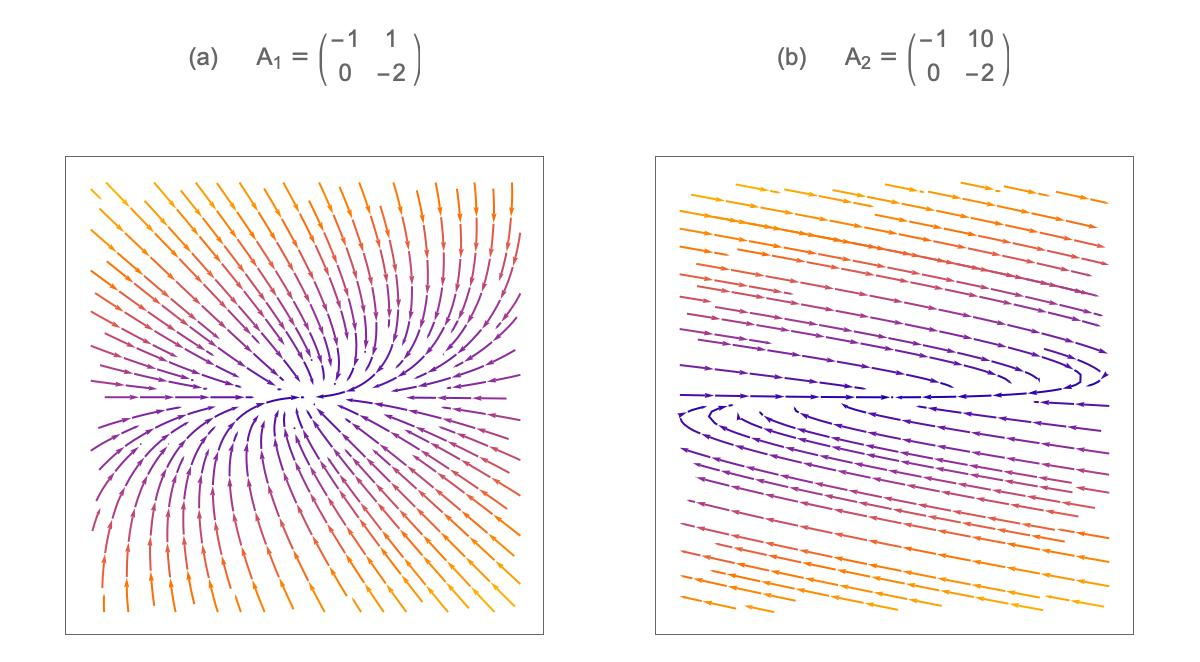
\includegraphics[width=0.8\textwidth]{figs/positive_reactivity_real_example}
	\caption{Phase portraits of two linear systems $x' = \textbf{A}x$ with the same eigenvalues  $\lambda = -1, -2$. (a) all trajectories decay monotonically in magnitude, (b) trajectories may initially move farther away from the origin before eventually limiting to 0. Example taken from \cite{neubertAlternativesResilienceMeasuring1997a}.}
\end{figure} 

\begin{definition}
	Let $\textbf{A}$ be the Jacobian as before. Let $\textbf{H} = \dfrac{\textbf{A}+\textbf{A}^T}{2}$ be its symmetric part. Since $\textbf{H}$ is a real symmetric matrix, it has real eigenvalues. \textbf{Reactivity} is equal to the maximum eigenvalue $\lambda_1(\textbf{H})$.  
	\(\qed\)
\end{definition}

If a linear system has positive reactivity, then there are arbitrarily small perturbations that will initially amplify, before eventually decaying to the sink. 